\documentclass{beamer}
%\usepackage{fullpage}
%\usepackage[left=2.8cm,right=2.2cm,top=2 cm,bottom=2 cm]{geometry}
\setbeamersize{text margin left=10pt,text margin right=10pt}
\usepackage{amsmath,amssymb}             % AMS Math
\usepackage[T1]{fontenc}
\usepackage[utf8]{inputenc}
\usepackage[french,english]{babel}
\usepackage{txfonts} 
\usepackage[]{graphicx}
\usepackage{multirow}
\usepackage{hyperref}

\renewcommand{\baselinestretch}{1.5}

\def\supit#1{\raisebox{0.8ex}{\small\it #1}\hspace{0.05em}}

\title[Vers une amélioration \\des résumés automatiques de textes \hspace*{2cm}  \textbf{\footnotesize  \insertframenumber/\inserttotalframenumber} ] %
{Vers une amélioration \\des résumés automatiques de textes} %:\\ Une méthode de score en utilisant le regroupement et l'apprentissage}
\institute{ %
École  nationale Supérieure d'Informatique (ESI, ex. INI), Algérie  %\\\supit{b} CERIST - Algérie %
}
\author[ARIES Abdelkrime (ESI 2014)] %
{ARIES Abdelkrime \\ {\footnotesize %
Encadré par: Pr. ZEGOUR Djamal Eddine\\%
Co-encadré par: Pr. HIDOUCI Khaled Walid}}

\titlegraphic{\includegraphics[height=1cm]{img/esi-logo.png}%\hspace*{4.75cm}~
}

\date{Etat d'avancement première année: 2013/2014} %\today

\usetheme{Warsaw} % Antibes Boadilla Warsaw

\beamertemplatenavigationsymbolsempty


\begin{document}

\selectlanguage {francais}

\begin{frame}[plain]
\maketitle
\end{frame}


\begin{frame}
\frametitle{Plan}
{\footnotesize \tableofcontents[hideothersubsections]}
\end{frame}

\section{Problématique}
\begin{frame}
\begin{center}
{\Huge Problématique}
\end{center}
\end{frame}

\subsection{Introduction}

\begin{frame}
\frametitle{Utilisation}

D’après \cite{75-borko-bernier}, les résumés :
\begin{itemize}
\item Permettent d'économiser le temps de lecture, en fournissant l’essentiel de
l’information.
\item Facilitent la sélection (des livre qu’on veut lire, par exemple);
\item Facilitent les recherches documentaires;
\item Améliorent l'efficacité d'indexation. 
Le résumé automatique de textes joue un rôle très importants dans le développement de systèmes de recherche d'information efficaces et performants \cite{03-allan-al}.
\end{itemize}

\end{frame}

\subsection{Description du problématique}

\begin{frame}
\frametitle{Aproche extractive vs. abstractive}

\begin{itemize}
\item Approche par extraction: extraction des unités pertinentes

\item Peut être indépendante de la langue et du genre de texte original
\begin{itemize}
\item Incohérence
\item Redondance
\end{itemize}
\end{itemize}

\begin{itemize}
\item Approche par abstraction: reformulation du contenu du texte original
\begin{itemize}
\item Absence des outils TALN performants
\item Difficile, et consomme trop de ressources mémoire et temps
\end{itemize}
\end{itemize}

\begin{itemize}
\item Techniques d'apprentissage
\begin{itemize}
\item Absence des corpus étiquetés
\end{itemize}
\end{itemize}

\end{frame}

\begin{frame}
\frametitle{Objectifs}

\begin{itemize}
\item \'Etudier les techniques de résumé automatique de textes, ainsi que celles de RI et de TALN.
\item Améliorer la solution proposée dans \cite{13-aries-al}.
\begin{itemize}
\item Appliquer des techniques d'apprentissage.
\item Appliquer les méthodes linguistiques.
\end{itemize}
\end{itemize}
\end{frame}

\subsection{Plan de travail}
\begin{frame}
\frametitle{Plan de travail}

\begin{enumerate}
\item \textbf{\color{red} Etat de l’art \textbf{(12 mois)}}
\item Proposition pour améliorer d’un premier papier \textbf{(12 mois)}
\item Validation avec deuxième papier \textbf{(16 mois)}
\item Rédaction de la thèse \textbf{(8 mois)}
\end{enumerate}
\end{frame}

\section{\'Etat de l'art}
\begin{frame}
\begin{center}
{\Huge \'Etat de l'art}
\end{center}
\end{frame}

\subsection{Résumé automatique}

\begin{frame}
\frametitle{Classification de résumé automatique}
Selon \cite{99-sparckjones,98-hovy-lin}:\\
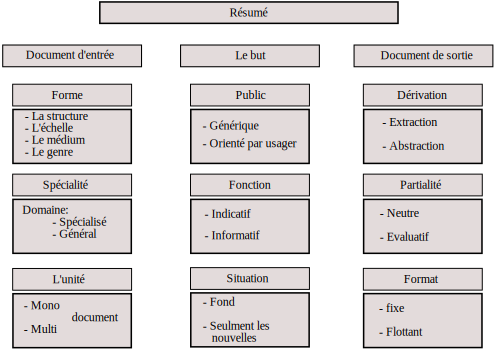
\includegraphics[width=120mm]{img/classif-resume.pdf} % % %[width=140mm]
\end{frame}

\begin{frame}
\frametitle{\'Evaluation de résumé automatique}
Selon \cite{01-mani}:\\
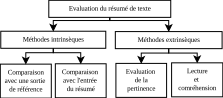
\includegraphics[width=120mm]{img/classif-eval.pdf} % % %[width=140mm]
\end{frame}

\subsection{Notre système (All Summarizer)}

\begin{frame}
\frametitle{Notre système (All Summarizer)}

\begin{itemize}
\item Méthode indépendante de la langue et du genre du document d'origine.
\item Moins de ressources: Mémoire, CPU (rapide).
\end{itemize}

\end{frame}

\begin{frame}
\frametitle{Notre système (All Summarizer)}

\begin{block}{Fonction de score}
$Score(P) = \sum_{1 \leq i \leq k} {\alpha_i * S_i(P)}$
\end{block}

Où:
\begin{itemize}
\item $k$ étant le nombre total de critères retenus pour calculer le score d'une phrase;
\item $S_i$ est la fonction calculant la valeur numérique d'un critère $ i $ appliqué à une phrase;
\item $\alpha_i$ est le coefficient associé au critère $ i $.
\end{itemize}

\end{frame}

\begin{frame}
\frametitle{Notre système (All Summarizer)}

\begin{itemize}
\item Un document contient plusieurs sujets (thèmes).
\item Les phrases similaires représentent, en général, le même sujet.
\item Un résumé est supposé être capable de représenter tous, ou la majorité des, sujets.
\end{itemize}
Donc:
\begin{block}{Notre but}
$ P(s_i \in \bigcap_{j} C_j | \overrightarrow{f}) = 
\prod_{j} P(s_i \in C_j | \overrightarrow{f}) $
\end{block}

\end{frame}

\begin{frame}
\frametitle{Notre système (All Summarizer)}
\framesubtitle{architecture générale}
\begin{center}
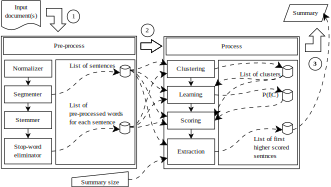
\includegraphics[width=100mm]{img/gnrl-arch.pdf}
\end{center}
\end{frame}

\begin{frame}
\frametitle{Notre système (All Summarizer)}
\framesubtitle{Regroupement}
\begin{center}
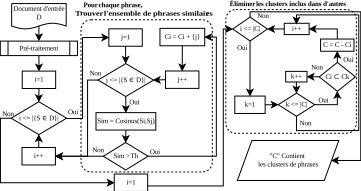
\includegraphics[width=110mm]{img/cluster.pdf}
\end{center}
\end{frame}

\begin{frame}
\frametitle{Notre système (All Summarizer)}
\framesubtitle{Classification comme fonction de notation}
\begin{block}{Notre but}
$ P(s_i \in \bigcap_{j} C_j | \overrightarrow{f}) = 
\prod_{j} P(s_i \in C_j | \overrightarrow{f}) $
\end{block}
\vfill
\begin{block}{Score de $ s_i $ dans toutes les classes, en utilisant tous les critères}
$ 
Score(s_i , \bigcap_{j} C_j , \overrightarrow{f}) = 
\prod_{j} \prod_{k} Score(s_i , C_j , f_k )
$
\end{block}

\end{frame}

\begin{frame}
\frametitle{Notre système (All Summarizer)}
\framesubtitle{Fonction d'apprentissage pour la classification de Bayes}

\begin{block}{Calcul de vraisemblance}
$ 
P(f = \phi | C) = \frac {F_{C\phi}}{\sum_{\phi'}{F_{C\phi'}}}
$
\end{block}
Où $\phi$ est une observation du critère $ f $ dans la classe $ C $. \\
$F_{C\phi}$ est le nombre de $\phi$ qui apparient dans la classe $ C $.

\vspace{10mm}

\begin{block}{Score de la phrase $ s $ dans la classe $ C $, en utilisant le critère $ f $}
$ 
Score(s , C , f ) = 1 + \sum_{\phi \in s} {P(f=\phi | C)}
$
\end{block}

\end{frame}

\begin{frame}
\frametitle{Notre système (All Summarizer)}
\framesubtitle{Code source}

Open source (GPL-v3) \\
\url{https://github.com/kariminf/AllSummarizer}
\end{frame}

\section{Nos contributions}
\begin{frame}
\begin{center}
{\Huge Nos contributions}\\
{\LARGE \textit{2013/2014}}
\end{center}
\end{frame}

\subsection{Résumé automatique multi-documents}

\begin{frame}
\frametitle{Résumé automatique multi-documents}
\framesubtitle{Deux propositions}
\begin{tabular}{cc}
Document = Cluster & \{phrase\} = Cluster \\
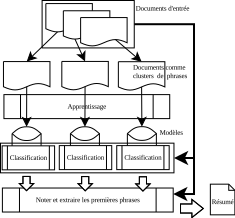
\includegraphics[width=55mm]{img/system1.pdf} &
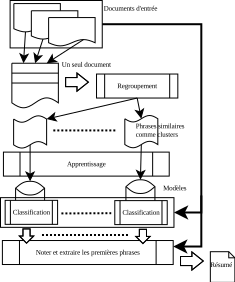
\includegraphics[width=45mm]{img/system2.pdf}
\end{tabular}
\end{frame}

\begin{frame}
\frametitle{Résumé automatique multi-documents}
\framesubtitle{Résultats d'évaluation: ROUGE-1}

\begin{block}{Résumé multi-documents - Methode1}
\begin{center}
\begin{tabular}{llll}
\hline \hline
$ f $	& \multicolumn{1}{c}{R}		& \multicolumn{1}{c}{P}	& \multicolumn{1}{c}{F1}	\\
\hline
U	& \textbf{0.3330}	& \textbf{0.3255}	& \textbf{0.3290} \\
B	& 0.3147	& 0.3109	& 0.3125	\\
UB	& 0.3191	& 0.3142	& 0.3164	 \\
\hline \hline
\end{tabular}
\end{center}
\end{block}
\end{frame}

\begin{frame}
\frametitle{Résumé automatique multi-documents}
\framesubtitle{Résultats d'évaluation: ROUGE-1}

\begin{block}{Résumé multi-documents - Methode2}
\scriptsize
\begin{center}
\begin{tabular}{lllllllll} 
\hline \hline
$ Th $	& \multicolumn{1}{c}{R}		& \multicolumn{1}{c}{P}	& \multicolumn{1}{c}{F1} && $ Th $	& \multicolumn{1}{c}{R}		& \multicolumn{1}{c}{P}	& \multicolumn{1}{c}{F1} \\
\hline
0.1	& 0.3399	& 0.3323	& 0.3359	&& 0.8	& 0.3480	& 0.3420	& 0.3448	 \\
0.2	& 0.3400	& 0.3323	& 0.3360	&& 0.9	& 0.3475	& 0.3407	& 0.3439	\\
0.3	& 0.3437	& 0.3368	& 0.3400	&& 1.0	& 0.3481	& 0.3413	& 0.3445	 \\
0.4	& \textbf{0.3514}	& \textbf{0.3447}	& \textbf{0.3478}	 &&&&& \\
0.5	& 0.3477	& 0.3415	& 0.3444	&&&&& \\
0.6	& 0.3467	& 0.3405	& 0.3434	&&&&& \\
0.7	& 0.3468	& 0.3410	& 0.3437	&&&&& \\
\hline \hline
\end{tabular}
\end{center}
\end{block}
Méthode 1: $ (R, P, F1)_{max}=(0.3330, 0.3255, 0.3290) $
\end{frame}

\subsection{Résumé automatique multi-lingue}

\begin{frame}
\frametitle{Résumé automatique multi-lingue}
\framesubtitle{Tester la performance dans le contexte multi-lingue}

\begin{block}{Critères de sélection}
\begin{center}
\begin{tabular}{lll}
\textit{TFU} && \textit{TFB} \\
\textit{POS} && \textit{LENG} \\
\end{tabular}
\end{center}
\end{block}

\begin{itemize}
\item Pour chaque combinaison des 4 critères (15 combinaisons)
\item Pour chaque langue \{Arabe, Chèque, Anglais, Français\}
\item Pour chaque seuil de regroupement \{0.1, 0.2, 0.3, 0.4, 0.5\}
\item Générer un résumé
\end{itemize}

\end{frame}


\begin{frame}
\frametitle{Résumé automatique multi-lingue}
\framesubtitle{Tester la performance dans le contexte multi-lingue}

\begin{center}
\includegraphics[width=95mm]{img/as-multiling-r2.pdf}
\end{center}

\end{frame}

\begin{frame}
\frametitle{Résumé automatique multi-lingue}
\framesubtitle{Tester la performance dans le contexte multi-lingue}

{\scriptsize
\begin{tabular*}{\textwidth}{@{\extracolsep{\fill}}lllll} 
\hline
\hline
Peer 			& 	Arabic 			& Czech 			& English 			& French			\\
\hline
\hline

CIST			& 0.10108			& 0.12585			& 0.12139			& 0.14077 			\\
CLASSY			& 0.15761			& 0.14316			& 0.17215			& 0.18360 			\\
JRC				& \textbf{0.19259}	& 0.14669			& 0.17352			& \textbf{0.19024} 	\\
LIF				& 0.15789			& 0.12794			& 0.15217			& 0.15266 			\\
SIEL IIITH		& -					& -					& 0.13610			& 0.11604 			\\
TALN UPF		& 0.11288			& -					& 0.10746			& 0.09748 			\\
UBSummarizer	& 0.07609			& 0.09308			& 0.09653			& 0.14138 			\\
UoEssex			& 0.12159			& -					& 0.12053			& - 				\\
\hline
Our system (th=0.07)		& 0.16237			& \textbf{0.16168}	& \textbf{0.17944}	& 0.18013 			\\
\hline
Baseline system	& 0.09794			& 0.10016			& 0.11023			& 0.11833 			\\
Topline system	& 0.29238			& 0.28926			& 0.25183			& 0.27478 			\\
\hline
\hline
\end{tabular*}
 }
\end{frame}


\begin{frame}
\frametitle{Résumé automatique multi-lingue}
\framesubtitle{Estimation du seuil de regroupement}

Dans notre évaluation précédente, il existe quelques limites:
\begin{itemize}
\item Le seuil doit être fixé au préalable.
\item Pour chaque document, il existe des seuils meilleures
\end{itemize}

$ th $ est utilisé avec les similarités entre les phrases\\
$ \Rightarrow  $ On peut estimer le seuil à partir des similarités entre phrases
{\scriptsize
\begin{itemize}
\item La moyenne arithmétique des similarités ;
\item La variance des similarités ;
\item Le mode;
\item La médiane.
\end{itemize}
}
\end{frame}

\begin{frame}
\frametitle{Résumé automatique multi-lingue}
\framesubtitle{Apprentissage du seuil de regroupement}
$ y = \frac{1}{1 + e^{-z}}  $ où $ z = b + \sum_{1}^{n} w_i x_i $
\begin{center}
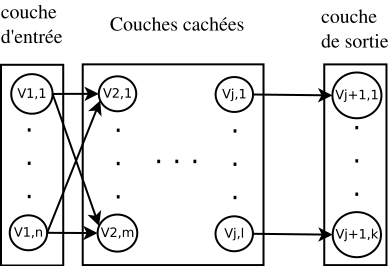
\includegraphics[width=60mm]{img/neural.pdf}
\end{center}
\textbf{nxmx...xjxk}
\end{frame}

\begin{frame}
\frametitle{Résumé automatique multi-lingue}
\framesubtitle{La préparation des données d'apprentissage}

Nous avons utilisé le corpus \textbf{Cmplg}:
\begin{itemize}
\item Pour chaque combinaison des 5 critères: tf-unigrams, tf-bigrams, position, taille-réelle, taille-après-pretraitement (31 combinaisons)
\item Pour chaque seuil de regroupement allant de 0 jusqu'à 1 avec un pas de 0.01 (101 seuils)
\item Pour chaque document des 181 documents
\item Générer un résumé
\end{itemize}
Donc, nous avons générer 566711 résumés. 

\end{frame}

\begin{frame}
\frametitle{Résumé automatique multi-lingue}
\framesubtitle{La préparation des données d'apprentissage}
{\small 
Nous avons utilisé le corpus \textbf{DUC2004-2}:
\begin{itemize}
\item Pour chaque combinaison des 5 critères: tf-unigrams, tf-bigrams, position, taille-réelle, taille-après-pretraitement (31 combinaisons)
\item Pour chaque $ th $ allant de 0 jusqu'à 0.25 avec un pas de 0.01 (26 seuils)
\item Pour chaque thème (50 thèmes) fusionner les 10 documents dans un seul document
\item Générer un résumé
\end{itemize}
Donc, nous avons généré 40300 résumés. }
\end{frame}

\begin{frame}
\frametitle{Résumé automatique multi-lingue}
\framesubtitle{\'Expérimentation}

Nous avons pris (8 cmplg, 2 duc) pour former les données de validation. \\
Le reste sont les données d'apprentissage.
\begin{itemize}
\item Pour chaque architecture, nous avons compté le temps nécessaire pour arriver à l'erreur de 0.001, ainsi que le nombre des itérations.
\item Pas d'amélioration de l'erreur: on sort.
\item Pour chaque architecture, 10 opérations d'apprentissage.
\item Pour chaque opération, nous avons compté le nombre des résultats valides (sur 10)
\end{itemize}
\end{frame}

\begin{frame}
\frametitle{Résumé automatique multi-lingue}
\framesubtitle{\'Expérimentation}
Les architectures testées, pour l’instant, sont:
\begin{itemize}
\item 4x4x1
\item 4x13x1
\item 4x13x13x1
\item 4x26x1
\item 4x52x1
\end{itemize}

\end{frame}

\begin{frame}
\frametitle{Résumé automatique multi-lingue}
\framesubtitle{\'Expérimentation}
Les buts de ces expérimentations sont:
\begin{itemize}
\item Choisir une architecture de réseaux de neurones, rapide dans l'étape d'apprentissage, et qui donne des bonnes résultats.
\item Choisir les critères (moyenne, médiane, etc.) utilisées pour entrainer le réseau de neurones (pour le seuil).
\end{itemize}
De même, on veut entrainer un autre réseau de neurones pour le choix des critères.
\end{frame}

\section{Conclusion et perspectives}
\begin{frame}
\frametitle{Conclusion et perspectives}

\begin{itemize}

\item Régler le problème de choix pour le seuil de regroupement, et des critères utilisées. 

\item Tester notre système dans le contexte de résumé automatique multi-documents et multi-lingue.

\item \color{red} Trouver un moyen pour représenter les phrases et les relations entre eux, dans le but de reformuler le résumé extrait et produire un autre qui est plus lisible.

\end{itemize}
\end{frame}

\begin{frame}
\frametitle{Fin ...}

\begin{center}
{\Huge Merci pour votre attention}
\end{center}
\end{frame}


%\subsection{Bibliography}
\frame[allowframebreaks]%
{\frametitle{Bibliography}
\tiny
\bibliography{cite}
\bibliographystyle{ESIbib} 
}


\end{document}

